\documentclass[parskip]{scrartcl}
\usepackage[margin=15mm,a3paper,landscape]{geometry}
\usepackage{tikz}

\begin{document}
\begin{tikzpicture}[x={(0.707cm,0.707cm)},z={(0cm,1cm)},y={(-0.866cm,0.5cm)}]
\draw[->] (-2,0,0) -- (2,0,0) node[right] {x};
\draw[->] (0,-2,0) -- (0,2,0) node[left] {y};
\draw[->] (0,0,-2) -- (0,0,12) node[above] {z};
\draw (1,0,0)
\foreach \z in {0,0.1,...,10}
{ -- ({cos(\z*100)},{sin(\z*100)},{\z})
};
\node[rotate=90,right=1cm] at (0,0,12) {normal rotation};
\end{tikzpicture}
\begin{tikzpicture}[x={(0.707cm,0.707cm)},z={(0cm,1cm)},y={(-0.866cm,0.5cm)}]
\draw[->] (-2,0,0) -- (2,0,0) node[right] {x};
\draw[->] (0,-2,0) -- (0,2,0) node[left] {y};
\draw[->] (0,0,-2) -- (0,0,12) node[above] {z};
\draw (1,0,0)
\foreach \z in {0,0.1,...,10}
{ -- ({cos(\z*200)},{sin(\z*100)},{\z})
};
\node[rotate=90,right=1cm] at (0,0,12) {WTF?};
\end{tikzpicture}
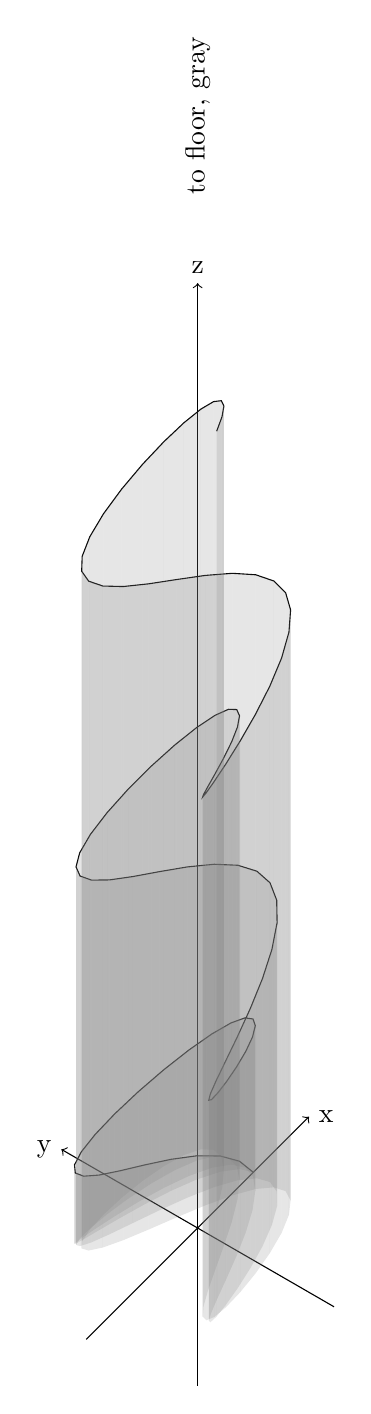
\begin{tikzpicture}[x={(0.707cm,0.707cm)},z={(0cm,1cm)},y={(-0.866cm,0.5cm)}]
\draw[->] (-2,0,0) -- (2,0,0) node[right] {x};
\draw[->] (0,-2,0) -- (0,2,0) node[left] {y};
\draw[->] (0,0,-2) -- (0,0,12) node[above] {z};
\draw (1,0,0)
\foreach \z in {0,0.1,...,10}
{ -- ({cos(\z*189)},{sin(\z*91)},{\z})
};
\foreach \z in {0,0.1,...,9.9}
{\fill[gray,opacity=0.2] ({cos(\z*189)},{sin(\z*91)},0) -- ({cos(\z*189)},{sin(\z*91)},{\z}) -- ({cos((\z+0.1)*189)},{sin((\z+0.1)*91)},{\z+0.1}) -- ({cos((\z+0.1)*189)},{sin((\z+0.1)*91)},0) -- cycle;
}
\node[rotate=90,right=1cm] at (0,0,12) {to floor, gray};
\end{tikzpicture}
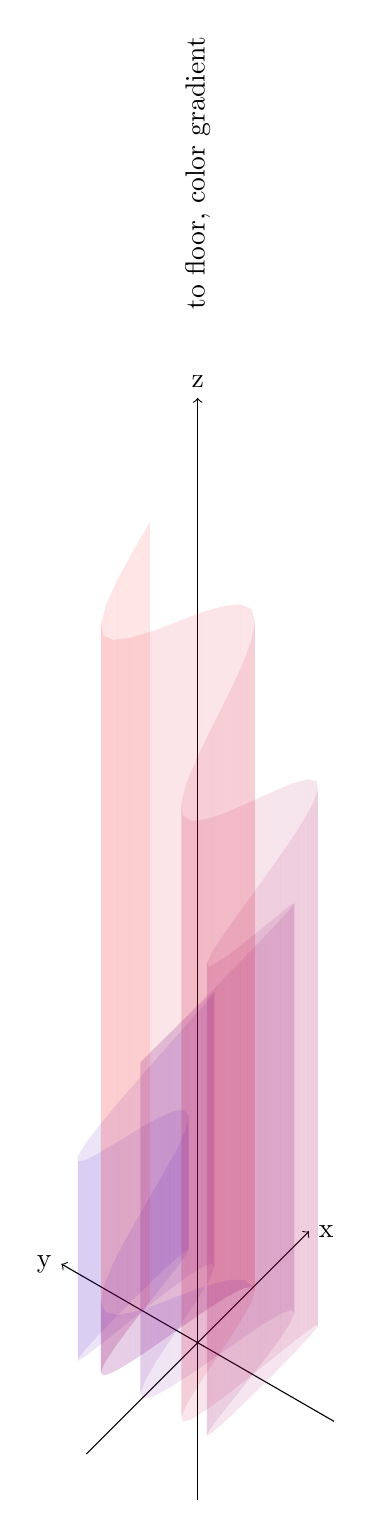
\begin{tikzpicture}[x={(0.707cm,0.707cm)},z={(0cm,1cm)},y={(-0.866cm,0.5cm)}]
\draw[->] (-2,0,0) -- (2,0,0) node[right] {x};
\draw[->] (0,-2,0) -- (0,2,0) node[left] {y};
\draw[->] (0,0,-2) -- (0,0,12) node[above] {z};
\foreach \z in {0,0.1,...,9.9}
{   \pgfmathtruncatemacro{\mycolorpercentage}{\z/0.099}
    \fill[red!\mycolorpercentage!blue,opacity=0.1] ({cos(\z*210)},{sin(\z*42)},0) -- ({cos(\z*210)},{sin(\z*42)},{\z}) -- ({cos((\z+0.1)*210)},{sin((\z+0.1)*42)},{\z+0.1}) -- ({cos((\z+0.1)*210)},{sin((\z+0.1)*42)},0) -- cycle;
}
\node[rotate=90,right=1cm] at (0,0,12) {to floor, color gradient};
\end{tikzpicture}
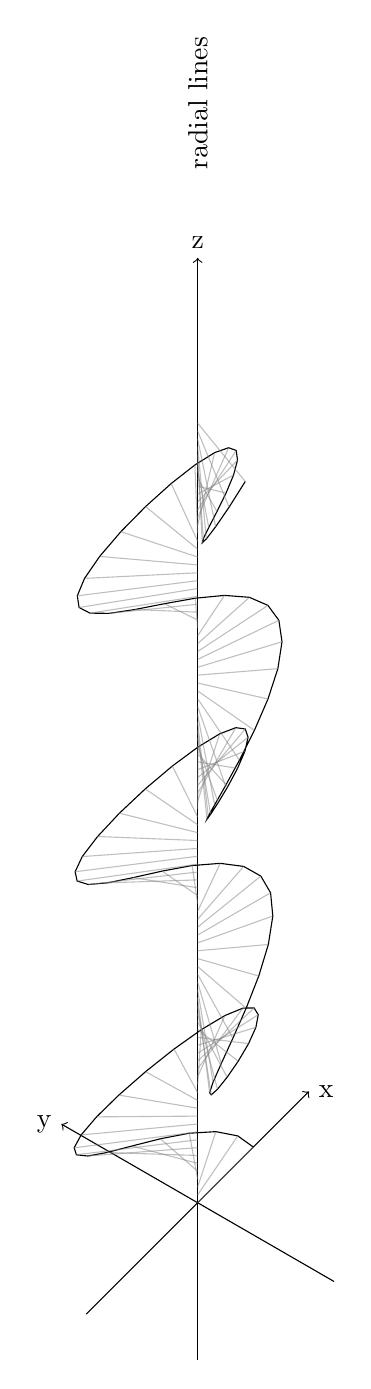
\begin{tikzpicture}[x={(0.707cm,0.707cm)},z={(0cm,1cm)},y={(-0.866cm,0.5cm)}]
\draw[->] (-2,0,0) -- (2,0,0) node[right] {x};
\draw[->] (0,-2,0) -- (0,2,0) node[left] {y};
\draw[->] (0,0,-2) -- (0,0,12) node[above] {z};
\draw (1,0,0)
\foreach \z in {0,0.1,...,10}
{ -- ({cos(\z*207)},{sin(\z*101)},{\z})
};
\foreach \z in {0,0.1,...,10}
{ \draw[opacity=0.5,gray] ({cos(\z*207)},{sin(\z*101)},{\z}) -- (0,0,\z);
}
\node[rotate=90,right=1cm] at (0,0,12) {radial lines};
\end{tikzpicture}
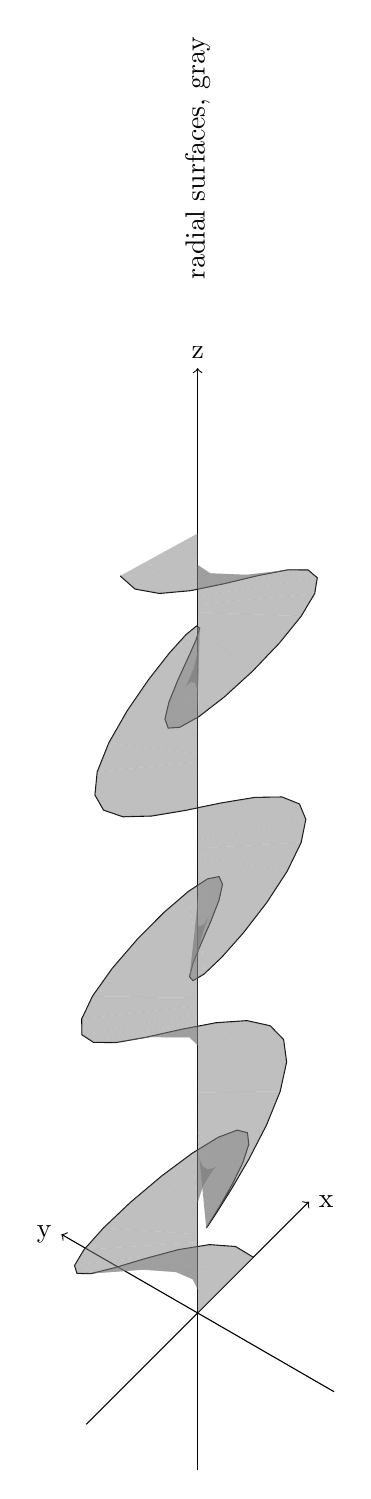
\begin{tikzpicture}[x={(0.707cm,0.707cm)},z={(0cm,1cm)},y={(-0.866cm,0.5cm)}]
\draw[->] (-2,0,0) -- (2,0,0) node[right] {x};
\draw[->] (0,-2,0) -- (0,2,0) node[left] {y};
\draw[->] (0,0,-2) -- (0,0,12) node[above] {z};
\draw (1,0,0)
\foreach \z in {0,0.1,...,10}
{ -- ({cos(\z*237)},{sin(\z*111)},{\z})
};
\foreach \z in {0,0.1,...,9.9}
{ \fill[opacity=0.5,gray] (0,0,\z) -- ({cos(\z*237)},{sin(\z*111)},{\z}) -- ({cos((\z+0.1)*237)},{sin((\z+0.1)*111)},{(\z+0.1)}) -- (0,0,{(\z+0.1)}) -- cycle;
}
\node[rotate=90,right=1cm] at (0,0,12) {radial surfaces, gray};
\end{tikzpicture}
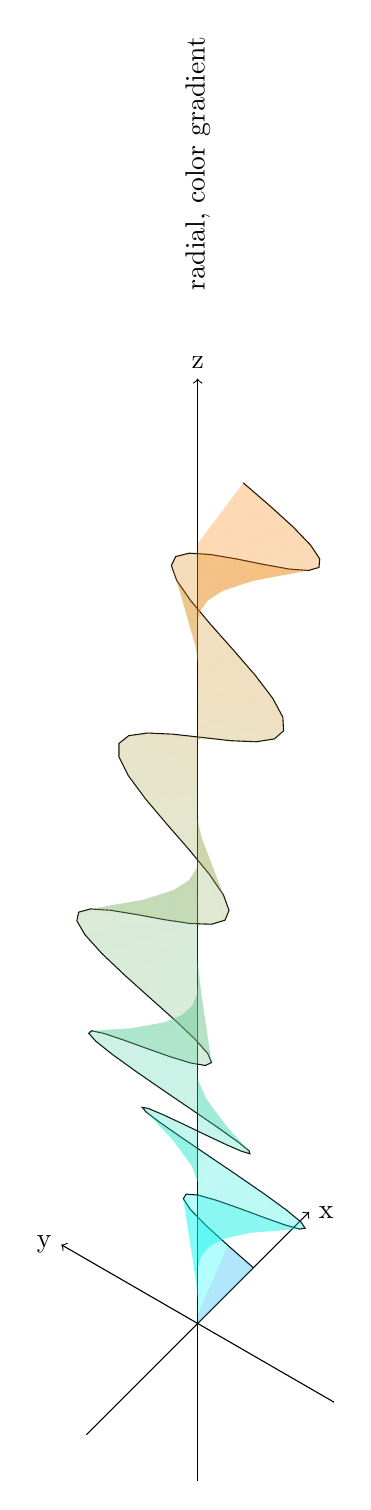
\begin{tikzpicture}[x={(0.707cm,0.707cm)},z={(0cm,1cm)},y={(-0.866cm,0.5cm)}]
\draw[->] (-2,0,0) -- (2,0,0) node[right] {x};
\draw[->] (0,-2,0) -- (0,2,0) node[left] {y};
\draw[->] (0,0,-2) -- (0,0,12) node[above] {z};
\draw (1,0,0)
\foreach \z in {0,0.1,...,10}
{ -- ({cos(\z*37)},{sin(\z*219)},{\z})
};
\foreach \z in {0,0.1,...,9.9}
{ \pgfmathtruncatemacro{\mycolorpercentage}{\z/0.099}
    \fill[opacity=0.3,orange!\mycolorpercentage!cyan] (0,0,\z) -- ({cos(\z*37)},{sin(\z*219)},{\z}) -- ({cos((\z+0.1)*37)},{sin((\z+0.1)*219)},{(\z+0.1)}) -- (0,0,{(\z+0.1)}) -- cycle;
}
\node[rotate=90,right=1cm] at (0,0,12) {radial, color gradient};
\end{tikzpicture}

\end{document}